\section{Differentialrechnung}

\subsection{Differenzierbarkeit}

\begin{definition}{Sekanten-Steigung und Differentialquotient}
    Sei $f$ eine Funktion und $\left[x_{0}, x_{0}+h\right]$ ein Intervall im Definitionsbereich von $f$. Der Quotient

    $$\frac{\Delta f}{\Delta x}=\frac{f\left(x_{0}+h\right)-f\left(x_{0}\right)}{h}$$

    heisst Differentialquotient von $f$.
\end{definition}

\begin{center}
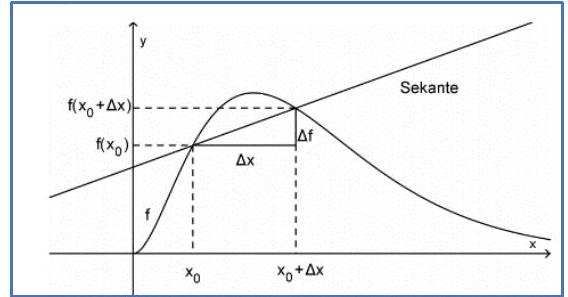
\includegraphics[scale=0.3]{2024_01_20_7bfda6c084929ccc01ffg-03.jpg}
\end{center}

\begin{definition}{Differenzierbarkeit}
    $f$ ist in $x_0$ \emph{differenzierbar}, falls der Grenzwert $\lim_{x \to x_0} \frac{f(x) -f(x_0)}{x -x_0}$
    existiert.

    Ist dies der Fall, wird der Grenzwert mit $f'(x)$ bezeichnet:
    $$
    f'(x_0) = \lim_{h \to 0}\frac{\Delta f}{\Delta x} = \lim_{h \to 0}\frac{f(x_0 + h) -f (x_0)}{h}
    $$
    Den Grenzwert selbst bezeichnet man als Ableitung.
    \tcblower
    Vereinfacht: Eine Funktion ist differenzierbar, falls die Kurve keine Knicke macht.
\end{definition}

\begin{formula}{Tangentengleichung}
    $$
    y=f^{\prime}\left(x_{0}\right) \cdot\left(x-x_{0}\right)+f\left(x_{0}\right)
    $$
\end{formula}

\begin{definition}{Stetige Differenzierbarkeit}
	Eine Funktion ist stetig differenzierbar, wenn sie differenzierbar ist und ihre Ableitungsfunktion stetig ist.
\end{definition}

\begin{definition}{n-fache Differenzierbarkeit}
	\begin{enumerate}
		\item Für $n \geq 2$ ist $f$ \emph{$n$-mal differenzierbar} in $D$ falls $f^{n-1}$ in $D$ differenzierbar ist. Dann ist $f^{(n)} \coloneqq \left(f^{(n-1)}\right)'$ und nennnt sich die $n$-te Ableitung von $f$.
		\item Die Funktion $f$ ist \emph{$n$-mal stetig differenzierbar} in $D$, falls sie $n$-mal differenzierbar ist und falls $f^{(n)}$ in $D$ stetig ist.
		\item Die Funktion $f$ ist in $D$ \emph{glatt}, falls sie $\forall n \geq 1$, $n$-mal differenzierbar ist.
	\end{enumerate}
\end{definition}

\begin{remark}
    Beispiele glatter Funktionen:
    \begin{itemize}
	    \item $\exp$, $\sin$, $\cos$, $\sinh$, $\cosh$, $\tanh$ sind glatt auf $\R$
	    \item Alle Polynome sind auf ganz $\R$ glatt
	    \item $\ln : ]0, + \infty[ \to \R$ ist glatt
    \end{itemize}
\end{remark}

\subsection{Ableitungen}

\subsubsection{Ableitungsregeln}

\begin{concept}{Ableitungsregeln}
    Seien $f,g: D \to \R$  differenzierbar. Dann gelten:
    \begin{itemize}
        \item Summe/Differenz: $$(f + g)'(x) = f'(x) + g'(x)$$
        \item Produkt: $$(f \cdot g)'(x) = f'(x)g(x) + f(x)g'(x)$$
        \item Quotient: $$\left(\frac{f}{g}\right)'(x) = \frac{f'(x) g(x) - f(x) g'(x)}{g(x)^2}$$
        \item Kettenregel: $$(g \circ f)' (x) = g'(f(x)) f'(x)$$
        \item Umkehrfunktion: $$\left(f^{-1}\right)'(y_0) = \frac{1}{f'(x)}$$
        \item Potenz/Logarithmus:
        $$(a^{f(x)})' = \ln(a) \cdot a^{f(x)} \cdot f'(x)$$
        $$(f(x)^{g(x)})' = f(x)^{g(x)} \cdot (\ln(f(x)) \cdot g(x))' =  f(x)^{g(x)} \cdot \left(\ln(f(x)) \cdot g'(x) + g(x) \cdot \frac{f'(x)}{f(x)}\right)$$
    \end{itemize}
\end{concept}

\subsubsection{Grundlegende Ableitungen}

\begin{formula}{Potenzfunktionen}
    $$f(x)=x^{n} \quad \Rightarrow \quad f^{\prime}(x)=n \cdot x^{n-1}$$
\end{formula}

\begin{formula}{Exponentialfunktionen}
    $$
    \begin{array}{ll}
    f(x)=a^{x} & f^{\prime}(x)=a^{x} \cdot \ln (a) \\
    f(x)=e^{x} & f^{\prime}(x)=e^{x}
    \end{array}
    $$
\end{formula}

\begin{formula}{Logarithmusfunktionen}
    $$
    \begin{array}{ll}
    f(x)=\ln (x) & f^{\prime}(x)=\frac{1}{x} \\
    f(x)=\log _{a}(x) & f^{\prime}(x)=\frac{1}{\ln (a) \cdot x}
    \end{array}
    $$
\end{formula}

\begin{formula}{Trigonometrische Funktionen}
    $$
    \begin{array}{ll}
    \sin'(x) = \cos(x) & \cos'(x) = -\sin(x) \\
    \tan'(x) = \frac{1}{\cos^{2}(x)} = 1+\tan^{2}(x) & \cot'(x) = -\frac{1}{\sin^{2}(x)} = -1-\cot^{2}(x)
    \end{array}
    $$
\end{formula}

\begin{formula}{Arkusfunktionen}
    $$
    \begin{aligned}
    \arcsin^{\prime}(x) & =\frac{1}{\sqrt{1-x^{2}}} \\
    \arccos^{\prime}(x) & =\frac{-1}{\sqrt{1-x^{2}}} \\
    \arctan^{\prime}(x) & =\frac{1}{1+x^{2}}
    \end{aligned}
    $$
\end{formula}

\begin{formula}{Hyperbolische Funktionen}
    $$
    \begin{array}{ll}
    \sinh'(x) = \cosh(x) & \cosh'(x) = \sinh(x)
    \end{array}
    $$
\end{formula}

\begin{remark}
    Für gerade $k$ gilt $\cosh (x)^{(k)}=\cosh (x)$ und für ungerade $k$ gilt $\cosh (x)^{(k)}=\sinh (x)$, analoges gilt für $\sinh$.
\end{remark}

\subsubsection{Weitere nützliche Ableitungen}

\begin{formula}{Weitere Ableitungen}
    $$
    \begin{array}{ll}
    \left(\frac{1}{x^n}\right)' = \frac{-n}{x^{n+1}} & \left(\sqrt[n]{x}\right)' = \frac{1}{n\sqrt[n]{x^{n-1}}} \\
    (x^x)' = x^x(1+\ln x) & (|x|)' = \sgn(x) \quad (x \neq 0)
    \end{array}
    $$
\end{formula}

\begin{center}
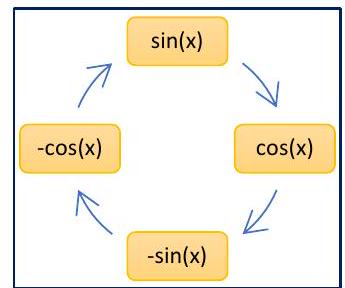
\includegraphics[scale=0.25]{2024_01_20_7bfda6c084929ccc01ffg-05.jpg}
\end{center}

\subsection{Höhere Ableitungen}

\begin{theorem}{Rechnen mit höheren Ableitungen}
	Sei $D \subseteq \R$, $n \geq 1$ und $f,g: D \to \R$ $n$-mal differenzierbar in $D$.
	\begin{enumerate}
		\item $f+g$ ist $n$-mal differenzierbar und $(f + g)^{(n)} = f^{(n)} + g^{(n)}$
		\item $f \cdot g$ ist $n$-mal differenzierbar und $(f \cdot g)^{(n)} = \sum_{k=0}^n \binom{n}{k} f^{(k)} g^{(n-k)}$ (Leibniz-Regel)
        \item $\frac{f}{g}$ ist $n$-mal differenzierbar falls $g(x) \neq 0, \forall x \in D$
        \item $(g \circ f)$ ist $n$-mal differenzierbar
	\end{enumerate}
\end{theorem}

\subsubsection{Zentrale Sätze der Ableitungsrechnung}

\begin{theorem}{Satz von Rolle}
    Sei $f:[a,b] \to \R$ stetig in $]a,b[$ differenzierbar. Erfüllt sie $f(a) = f(b)$ so gibt es $\xi \in ]a,b[$ mit $f'(\xi) = 0$.

    \tcblower
    $\xi$ bezeichnet eine Extremalstelle im Intervall $]a,b[$.
\end{theorem}

\begin{theorem}{Lagrange (Mittelwertsatz)}
    Sei $f:[a,b] \to \R$ stetig mit $f$ in $]a,b[$ differenzierbar. Dann gibt es $\xi \in ]a,b[$ mit
    $$f(b) - f(a) = f'(\xi) (b-a)$$

    \tcblower
    $f'(\xi)$ ist die Steigung der Sekante zwischen $(a, f(a))$ und $(b, f(b))$:
    $$f'(\xi) = \frac{f(b) - f(a)}{b - a}$$
\end{theorem}

\begin{theorem}{l'Hospital}
    Seien $f,g : [a,b] \to \R$ stetig und in $]a,b[$ differenzierbar. Dann gibt es $\xi \in ]a,b[$ mit
    $$g'(\xi)\left(f(b) - f(a)\right) = f'(\xi) \left(g(b) - g(a)\right)$$

    Falls $g'(x) \neq 0 \quad \forall x \in ]a,b[$ folgt $g(a) \neq g(b)$ und
    $$\frac{f(b) - f(a)}{g(b) - g(a)} = \frac{f'(\xi)}{g'(\xi)}$$
\end{theorem}

\subsection{Kurvendiskussion}

\subsubsection{Monotonie und Krümmung}

\begin{definition}{Monotonie}
    Sei $y=f(x)$ eine differenzierbare Funktion in $D$ mit $x_{0} \in D$.
    \begin{itemize}
        \item $f'(x_{0}) = 0$ $\Rightarrow$ $f$ konstant, bzw. horizontale Tangente
        \item $f'(x_{0}) > 0$ $\Rightarrow$ $f$ streng monoton wachsend
        \item $f'(x_{0}) < 0$ $\Rightarrow$ $f$ streng monoton fallend
    \end{itemize}
\end{definition}

\begin{theorem}{Krümmung}
    Zusammenhang zwischen 2. Ableitung und Krümmung:
    \begin{itemize}
      \item $f^{\prime \prime}\left(x_{0}\right)>0$ $\Rightarrow$ Konvex (linksgekrümmt, nach oben geöffnet)
      \item $f^{\prime \prime}\left(x_{0}\right)<0$ $\Rightarrow$ Konkav (rechtsgekrümmt, nach unten geöffnet)
      \item $f^{\prime \prime}\left(x_{0}\right)=0$ $\Rightarrow$ Keine eindeutige Krümmung
    \end{itemize}
\end{theorem}

\begin{remark}
    Die Summe zweier konvexer Funktionen ist konvex. (Für konkave Funktionen gilt dies analog.)
\end{remark}

\begin{center}
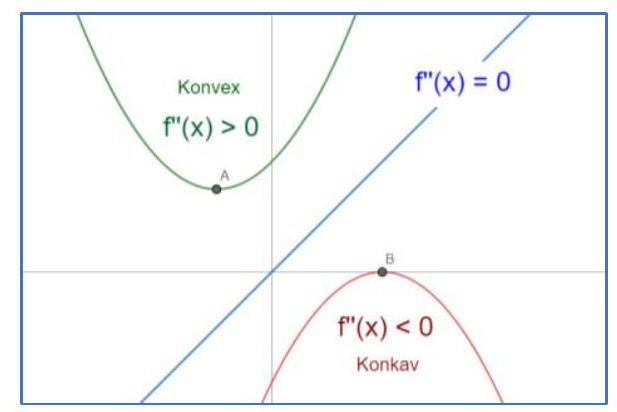
\includegraphics[scale=0.2]{2024_01_20_7bfda6c084929ccc01ffg-07.jpg}
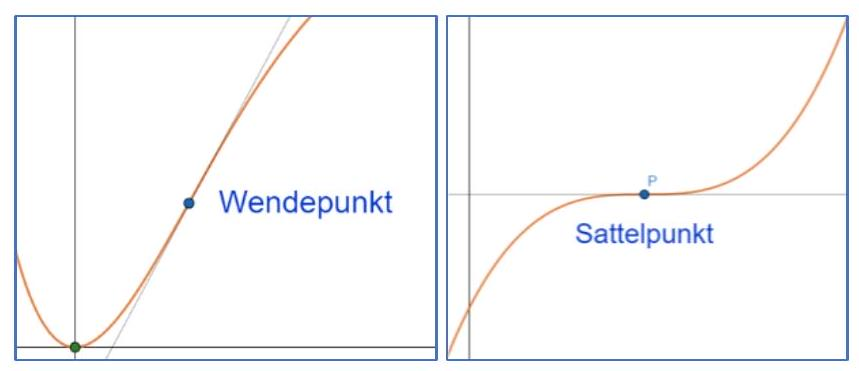
\includegraphics[scale=0.15]{2024_01_20_7bfda6c084929ccc01ffg-08.jpg}
\end{center}

\subsubsection{Relative Extrema}

\begin{definition}{Relative Extrema}
    \begin{itemize}
      \item Relative Extremal-Stelle $x_0$ $\Longrightarrow$ Minimal-/Maximalstelle
      \item Relatives Extremum $y_0$ $\Longrightarrow$ Maximum/Minimum
      \item Relativer Extremal-Punkt $P_0 = (x_0, y_0)$ $\Longrightarrow$ Hoch-/Tiefpunkt
    \end{itemize}
\end{definition}

\begin{center}
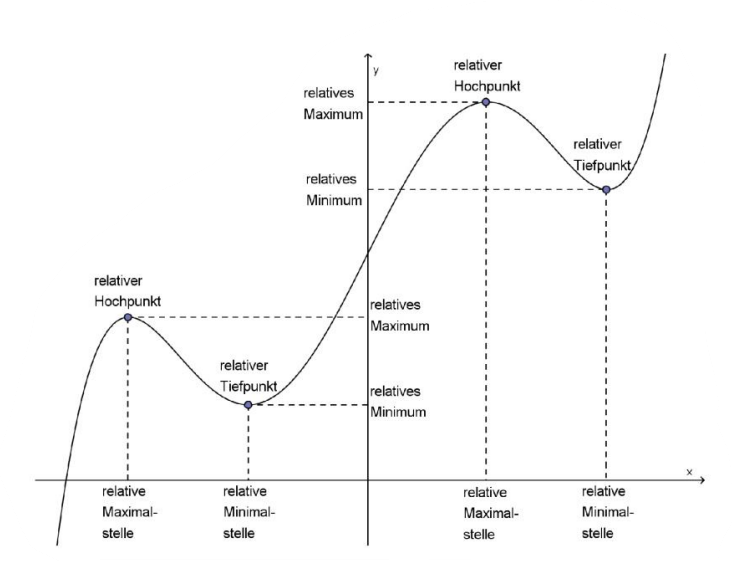
\includegraphics[scale=0.45]{relative maxima.png}
\end{center}

\begin{KR}{Vorgehen relative Extrema}
    Bestimmung relativer Extrema von $f(x) = y$:
    \begin{enumerate}
	    \item Bestimme $f'(x)$ (Erste Ableitung)
	    \item Bestimme Nullstellen von $f'(x)$: $f'(x) = 0 \Rightarrow x$ lokales Extremum
	    \item Bestimme $f''(x)$ (Zweite Ableitung)
		    \begin{itemize}
			    \item $f''(x) = 0$ $\Rightarrow$ siehe Allgemeines Kriterium
			    \item $f''(x) < 0$ $\Rightarrow$ relatives Maximum (Hochpunkt)
			    \item $f''(x) > 0$ $\Rightarrow$ relatives Minimum (Tiefpunkt)
		    \end{itemize}
        \item In Gleichung $f(x) = y$ einsetzen für Punkt $P(x, y)$
    \end{enumerate}
\end{KR}

\begin{example}
    $$f(x)=x^{5}-\frac{65}{3} x^{3}+180 x$$

    \begin{enumerate}
        \item $f'(x)=5 x^{4}-65 x^{2}+180$
        \item $f'(x)=0 \Rightarrow x_{0}=2 \pm \sqrt{3}$
        \item $f''(x)=20 x^{3}-130 x$
        \item Einsetzen:
            \begin{itemize}
              \item $f^{\prime \prime}(2-\sqrt{3})=-34 < 0 \Rightarrow$ Maximum
              \item $f^{\prime \prime}(2+\sqrt{3})=554 > 0 \Rightarrow$ Minimum
            \end{itemize}
        \item Hochpunkt/Tiefpunkt: $P\left(x_{0}, f(x_0)\right)$
    \end{enumerate}
\end{example}

\subsubsection{Wende- und Sattelpunkte}

\begin{definition}{Wende- und Sattelpunkte}
    Als Wendepunkte werden Punkte bezeichnet bei denen sich der Drehsinn (die Krümmung) ändert.

    Wendepunkte mit horizontaler Tangente werden als Sattelpunkte oder Terrassenpunkte bezeichnet.

    Die Tangente an einem Wendepunkt heisst Wendetangente.
\end{definition}

\begin{KR}{Berechnung Wendepunkte}
    Ermittlung durch Lösen der Gleichung $f^{\prime \prime}(x)=0 \rightarrow x_{0}$.

    Bedingungen (sei $y=f(x)$ dreimal differenzierbar):
    \begin{itemize}
      \item $f^{\prime \prime}\left(x_{0}\right)=0$
      \item $f^{(3)}\left(x_{0}\right) \neq 0$ $\Rightarrow$ Wendepunkt
      \item Falls zusätzlich $f^{\prime}\left(x_{0}\right)=0$ $\Rightarrow$ Sattelpunkt
    \end{itemize}
\end{KR}

\begin{concept}{Allgemeines Kriterium}
    Sei $f(x)$ eine genügend oft differenzierbare Funktion mit $f^{\prime}\left(x_{0}\right)=0$.

    Sei $n$ die Ordnung der ersten nicht verschwindenden Ableitung von $f(x)$ an der Stelle $x_{0}$:
    \begin{itemize}
      \item $f^{\prime}\left(x_{0}\right)=f^{\prime \prime}\left(x_{0}\right)=\cdots=f^{(n-1)}\left(x_{0}\right)=0$
      \item $f^{(n)}\left(x_{0}\right) \neq 0$
    \end{itemize}

    Schlussfolgerungen:
    \begin{itemize}
        \item Wenn $n$ gerade, dann gibt es ein relatives Extremum bei $x_0$
        \item Wenn $n$ ungerade, dann hat $f(x)$ an der Stelle $x_{0}$ einen Wendepunkt und damit einen Sattelpunkt
    \end{itemize}
\end{concept}

\begin{KR}{Vorgehen Wende- und Sattelpunkte}
    \begin{enumerate}
      \item Erste, zweite und dritte Ableitung bestimmen
      \item Wendepunkt bestimmen:
        \begin{itemize}
          \item $f^{\prime \prime}\left(x_{0}\right)=0 \rightarrow x_{0}$
          \item $f^{(3)}\left(x_{0}\right) \neq 0$ $\Rightarrow$ Wendepunkt
        \end{itemize}
      \item Sattelpunkte bestimmen (falls $f'(x_0) = 0$):
        \begin{itemize}
          \item $f^{\prime}\left(x_{0}\right)=0$
          \item $f^{\prime \prime}\left(x_{0}\right)=0$
          \item $f^{(n)}\left(x_{0}\right) \neq 0$ für kleinste $n \geq 3$
          \item $n$ gerade $\Rightarrow$ relatives Extremum
          \item $n$ ungerade $\Rightarrow$ Sattelpunkt
        \end{itemize}
      \item $x_{0}$ in ursprüngliche Gleichung einsetzen für Punkt $P(x_0, f(x_0))$
    \end{enumerate}
\end{KR}

\subsubsection{Allgemeine Kurvendiskussion}

\begin{KR}{Vorgehen Kurvendiskussion}
    Kurvendiskussion für eine Funktion $y=f(x)$:
    \begin{enumerate}
      \item Definitionsbereich bestimmen
      \item Symmetrie prüfen (gerade/ungerade Funktion)
      \item Schnittpunkte mit den Koordinatenachsen
        \begin{itemize}
            \item Nullstellen: $f(x) = 0$
            \item Y-Achsenabschnitt: $f(0)$
        \end{itemize}
      \item Verhalten für $x \rightarrow \pm\infty$ (Asymptoten)
      \item Relative Extrema inkl. Typbestimmung
      \item Wendepunkte, insbesondere Sattelpunkte
      \item Graph skizzieren
    \end{enumerate}
\end{KR}

\begin{concept}{Graphen skizzieren}
    Beispiel: $y=0.5 \cdot\left(x^{2}-5 x+4\right)$

    Nullstellen:
    \begin{itemize}
      \item $0=0.5 \cdot(x-1) \cdot(x-4) \Rightarrow x_{1}=1, x_{2}=4$
    \end{itemize}

    Y-Achsenabschnitt:
    \begin{itemize}
      \item $y=0.5 \cdot x^{2}-2.5 \cdot x+2 \Rightarrow y_{0}=2$
    \end{itemize}

    \begin{center}
    \includegraphics[width=0.8\linewidth]{2024_01_20_7bfda6c084929ccc01ffg-09.jpg}
    \end{center}

    Relative Extrema ($n$ gerade, $n>1$):
    \begin{itemize}
      \item Positiv: $y=0.5 \cdot(x-3)^{n} \cdot(\ldots)+3 \Rightarrow$ Tiefpunkt
      \item Negativ: $y=-0.5 \cdot(x-3)^{n} \cdot(\ldots)+1 \Rightarrow$ Hochpunkt
    \end{itemize}

    Wendepunkte ($n$ ungerade, $n>2$):
    \begin{itemize}
      \item $y=0.5 \cdot(x-3)^{n} \cdot(\ldots)+c \Rightarrow$ Wendepunkt
    \end{itemize}
\end{concept}

\subsection{Potenzreihen und Taylor-Reihen}

\begin{theorem}{Potenzreihen}
	Sei $\sum_{k=0}^\infty c_k x^k$ eine Potenzreihe mit positivem Konvergenzradius $\rho > 0$. Dann ist
    $$f(x) = \sum_{k=0}^\infty c_k (x-x_0)^k$$
    auf $]x_0 - \rho, x_0 + \rho[$ differenzierbar und
    $$f'(x) = \sum_{k=1}^\infty k c_k (x - x_0)^{k-1}$$
    für alle $x \in ]x_0 - \rho, x_0 + \rho[$.
\end{theorem}

\begin{remark}
    Jede glatte Funktion kann als Potenzreihe angenähert werden. Dafür brauchen wir ein sogenanntes Taylor-Polynom (oder Taylorreihen). Die trigonometrischen Funktionen sind genau solche Taylorreihen.
\end{remark}

\begin{theorem}[important]{Taylor-Approximation}
	Sei $f: [c,d] \to \R$ stetig und in $]c,d[$ $(n+1)$-mal differenzierbar.
	Sei $c<a<d$.
	Für alle $x \in [c,d]$ gibt es $\xi$ zwischen $x$ und $a$, sodass
	\begin{equation*}
		f(x) = \sum_{k=0}^n \frac{f^{(k)} (a)}{k!} (x - a)^k + \frac{f^{(n+1)} (\xi)}{(n+1)!} (x - a)^{n+1}
	\end{equation*}
\end{theorem}

\begin{remark}
    Der letzte Term $\frac{f^{(n+1)} (\xi)}{(n+1)!} (x - a)^{n+1}$ wird meist zur Fehlerabschätzung innerhalb eines Bereiches von $a$ verwendet. Man nimmt daher den Wert von $\xi \in ]a, x[$, so dass der Fehlerterm am grössten ist.
\end{remark}

\begin{corollary}{Bekannte Taylorreihen}
    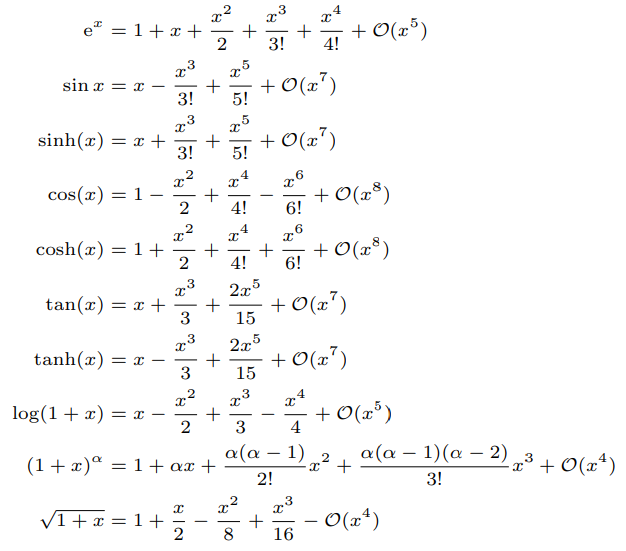
\includegraphics[scale=0.5]{bekannte_taylorreihen.png}
\end{corollary}

\subsubsection{Konvergenz mit Taylorreihen}

\begin{center}
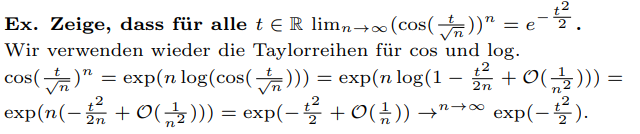
\includegraphics[scale=0.5]{5.png}
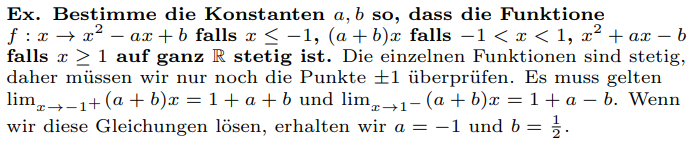
\includegraphics[scale=0.5]{4.png}
\end{center}
